%---------------------------------------------------------------------
% Appendix E: held-out evaluation of the calibration methods
% Numbers from results/experiments/compensation/full_comparison (run 2026-10-13T09:39:49),
% calibration run results/experiments/compensation/calibration/Water/Water_water_final_stereo.yaml
%---------------------------------------------------------------------

\chapter{Held-out evaluation: recordings, splits and image zones}
\label{app:heldout}

This appendix lists the exact data behind the held-out comparison of the calibration methods: which underwater
recordings and frames were used, which recordings each split held out, and how every board corner was assigned
to an image zone and a distance band. The comparison is produced by
\texttt{src/experiments/compensation/run\_comparison.py} with the configuration \texttt{config\_full.json};
the list of splits is also saved in \texttt{run\_info.json} beside the results.

\section{Underwater recordings and frames}
\label{app:heldout:recordings}

The underwater calibration data are eight recordings of the Kalibr AprilGrid (AprilTag 36h11, 35.36~mm tags,
$10\times7$), each a sweep of the board towards and away from the rig at one tilt. One stereo frame was extracted
per nominal distance; the nominal distance in centimetres is the number in the file name
(\texttt{c1\_Left\_100.png} is the left image at a nominal 100~cm). The corners were detected once by
\texttt{Calibration.py} with the \texttt{water\_final} detector preset on the gray channel. Only the images and
tags that run kept after its outlier rejection are used, so a camera can have fewer frames than its recording.
The measured distance is from the camera to the board centre, from each image's board pose in that calibration.

\begin{table}[H]
\centering
\caption{The eight underwater recordings: frames kept per camera (nominal distances in cm), measured
camera-to-board distance range of the left camera, and stereo pairs (frames both cameras kept with at least 10
tags in common).}
\label{tab:app:recordings}
\small
\begin{tabular}{lllcc}
\toprule
Recording & Left frames (nominal cm) & Right frames (nominal cm) & Left distance (mm) & Pairs \\
\midrule
\texttt{Water\_C1\_frames} & 11 (50--150)          & 11 (50--150)          & 232--1221 & 11 \\
\texttt{Water\_C3\_frames} & 11 (50--150)          & 11 (50--150)          & 262--1234 & 10 \\
\texttt{Water\_C4\_frames} & 10 (50--140)          & 10 (50--140)          & 363--1252 & 10 \\
\texttt{Water\_C5\_frames} & 10 (60--150)          & 11 (50--150)          & 484--1378 & 10 \\
\texttt{Water\_C6\_frames} &  8 (70--140)          &  8 (70--140)          & 621--1318 &  7 \\
\texttt{Water\_L1\_Frames} & 12 (40--150)          & 10 (60--150)          & 353--1367 & 10 \\
\texttt{Water\_L3\_Frames} & 11 (50--150)          & 10 (60--150)          & 441--1377 & 10 \\
\texttt{Water\_L5\_Frames} & 11 (50--150)          &  9 (70--150)          & 484--1416 &  9 \\
\midrule
Total                      & 84                    & 80                    & 232--1416 & 77 \\
\bottomrule
\end{tabular}
\end{table}

Within each range in Table~\ref{tab:app:recordings} the frames are at every 10~cm. The images of
\texttt{Water\_L1\_Frames} are named \texttt{c1\_\ldots} on disk; they are a separate recording from
\texttt{Water\_C1\_frames}. Altogether the left camera contributes 18\,772 board corners and the right camera
18\,436.

\section{Held-out splits}
\label{app:heldout:splits}

Frames within one recording are near neighbours, so holding out single frames would test a model on almost the
data it was fitted to. Instead, whole recordings are held out: every combination of two of the eight recordings
($\binom{8}{2} = 28$ splits). In each split every technique is fitted on the six remaining recordings and scored
on all the kept frames of the two held-out ones. Every recording is therefore held out in 7 splits and used for
training in the other 21, and every held-out frame is scored by a model that never saw its recording. All
techniques are scored on exactly the same held-out corners in every split.

\begin{table}[H]
\centering
\caption{The 28 splits: the two held-out (test) recordings, and the held-out left frames, right frames and
stereo pairs. The training set of each split is the other six recordings.}
\label{tab:app:splits}
\small
\begin{tabular}{rlccc@{\hspace{2.5em}}rlccc}
\toprule
Split & Held out & L & R & Pairs & Split & Held out & L & R & Pairs \\
\midrule
 0 & C1, C3 & 22 & 22 & 21 & 14 & C4, C6 & 18 & 18 & 17 \\
 1 & C1, C4 & 21 & 21 & 21 & 15 & C4, L1 & 22 & 20 & 20 \\
 2 & C1, C5 & 21 & 22 & 21 & 16 & C4, L3 & 21 & 20 & 20 \\
 3 & C1, C6 & 19 & 19 & 18 & 17 & C4, L5 & 21 & 19 & 19 \\
 4 & C1, L1 & 23 & 21 & 21 & 18 & C5, C6 & 18 & 19 & 17 \\
 5 & C1, L3 & 22 & 21 & 21 & 19 & C5, L1 & 22 & 21 & 20 \\
 6 & C1, L5 & 22 & 20 & 20 & 20 & C5, L3 & 21 & 21 & 20 \\
 7 & C3, C4 & 21 & 21 & 20 & 21 & C5, L5 & 21 & 20 & 19 \\
 8 & C3, C5 & 21 & 22 & 20 & 22 & C6, L1 & 20 & 18 & 17 \\
 9 & C3, C6 & 19 & 19 & 17 & 23 & C6, L3 & 19 & 18 & 17 \\
10 & C3, L1 & 23 & 21 & 20 & 24 & C6, L5 & 19 & 17 & 16 \\
11 & C3, L3 & 22 & 21 & 20 & 25 & L1, L3 & 23 & 20 & 20 \\
12 & C3, L5 & 22 & 20 & 19 & 26 & L1, L5 & 23 & 19 & 19 \\
13 & C4, C5 & 20 & 21 & 20 & 27 & L3, L5 & 22 & 19 & 19 \\
\bottomrule
\end{tabular}
\end{table}

\subsection{How a held-out frame is scored}
\label{subsec:appE.heldout_scoring}
For a held-out image, the technique's intrinsics are fixed and only the board pose $(R,\mathbf{t})$ is fitted, by
minimising the pixel distance between the detected corners $\mathbf{u}_i$ and their projections
$\hat{\mathbf{u}}_i = \pi(R\mathbf{X}_i + \mathbf{t})$, where $\mathbf{X}_i$ are the known board coordinates and
$\pi$ is the technique's camera model. The residual of corner $i$ is $\mathbf{e}_i = \mathbf{u}_i -
\hat{\mathbf{u}}_i$, and the held-out error of a split over a set $S$ of its held-out corners is
\begin{equation}
  \mathrm{RMS}_S = \sqrt{\frac{1}{|S|}\sum_{i\in S} \lVert \mathbf{e}_i \rVert^2 }.
\end{equation}
$S$ is all held-out corners for the overall figure, or only those in one image zone or distance band
(Sections~\ref{app:heldout:zones} and~\ref{app:heldout:bands}). Each metric is computed once per split, and the
tables report the mean over the 28 splits with the 2.5--97.5 percentile range of the 28 values. Because the pose
is fitted to the corners it is scored on, part of any model error is absorbed into it, so the held-out RMS is a
lower bound on the error at an unknown pose.

\section{Normalised radius and image zones}
\label{app:heldout:zones}

Lens distortion and refraction errors grow with distance from the optical axis, so the residuals are also
reported by where the corner lies in the image. The reference point is the principal point $(c_x, c_y)$ of the
technique being scored, the point where the optical axis meets the image. The pixel distance of a corner at
$(u, v)$ from it is divided by the distance from the principal point to the farthest of the four image corners:
\begin{equation}
  r = \frac{\sqrt{(u - c_x)^2 + (v - c_y)^2}}{R_{\max}}, \qquad
  R_{\max} = \max_{(x,\,y)\,\in\,\{0,\,W\}\times\{0,\,H\}} \sqrt{(x - c_x)^2 + (y - c_y)^2},
  \label{eq:app:radius}
\end{equation}
with $W \times H = 1600 \times 1200$~px. So $r = 0$ at the principal point and $r = 1$ at the farthest image
corner. Normalising by the image rather than using pixels makes the zone boundaries mean the same thing for every
technique, whose principal points differ by a few pixels, and for any image resolution. The image is then split
into three concentric zones:
\begin{equation}
  \text{centre: } r < 0.33, \qquad \text{mid: } 0.33 \le r < 0.66, \qquad \text{outer: } r \ge 0.66 .
\end{equation}

Table~\ref{tab:app:zones} gives the values for the underwater Brown-Conrady fit on all recordings. The other
techniques' principal points are within 4~px of these, so their zone boundaries move by less than 4~px.

\begin{table}[H]
\centering
\caption{Principal point, $R_{\max}$ and zone boundaries in pixels (underwater Brown-Conrady), and the share of
held-out corners in each zone and distance band, pooled over all splits.}
\label{tab:app:zones}
\small
\begin{tabular}{lcc}
\toprule
 & Left camera & Right camera \\
\midrule
Principal point $(c_x, c_y)$ (px)        & (792.7, 642.2) & (769.8, 630.6) \\
$R_{\max}$ (px), farthest corner          & 1031.6, $(1600, 0)$ & 1042.6, $(1600, 0)$ \\
Centre / mid boundary, $0.33R_{\max}$ (px) & 340 & 344 \\
Mid / outer boundary, $0.66R_{\max}$ (px)  & 681 & 688 \\
\midrule
Corners in centre / mid / outer (\%)     & 67.0 / 29.9 / 3.1 & 57.7 / 38.2 / 4.1 \\
Corners near / far / between (\%)        & 42.6 / 35.9 / 21.5 & 34.4 / 41.8 / 23.8 \\
\bottomrule
\end{tabular}
\end{table}

\begin{figure}[H]
\centering
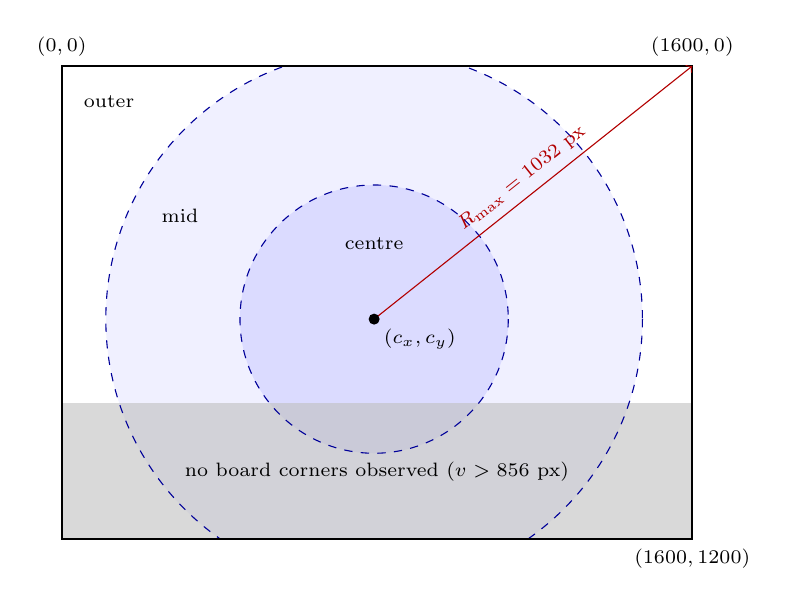
\begin{tikzpicture}[x=0.005cm, y=-0.005cm]
  \begin{scope}
    \clip (0,0) rectangle (1600,1200);
    \fill[blue!6] (792.7,642.2) circle (680.9);
    \fill[blue!14] (792.7,642.2) circle (340.4);
    % unobserved part of the image (no board corner below v = 856 px in either camera)
    \fill[black!25, opacity=0.6] (0,856) rectangle (1600,1200);
    \draw[blue!60!black, dashed] (792.7,642.2) circle (340.4);
    \draw[blue!60!black, dashed] (792.7,642.2) circle (680.9);
  \end{scope}
  \draw[thick] (0,0) rectangle (1600,1200);
  \draw[->, red!70!black] (792.7,642.2) -- node[pos=0.5, above, sloped, font=\scriptsize] {$R_{\max} = 1032$~px} (1600,0);
  \fill (792.7,642.2) circle (14);
  \node[font=\scriptsize, below right] at (792.7,642.2) {$(c_x, c_y)$};
  \node[font=\scriptsize] at (792.7,450) {centre};
  \node[font=\scriptsize] at (300,380) {mid};
  \node[font=\scriptsize] at (120,90) {outer};
  \node[font=\scriptsize] at (800,1030) {no board corners observed ($v > 856$~px)};
  \node[font=\scriptsize, above] at (0,0) {$(0,0)$};
  \node[font=\scriptsize, above] at (1600,0) {$(1600,0)$};
  \node[font=\scriptsize, below] at (1600,1200) {$(1600,1200)$};
\end{tikzpicture}
\caption{The left image ($1600\times1200$~px) divided into the centre ($r<0.33$), mid ($0.33\le r<0.66$) and
outer ($r\ge0.66$) zones about the principal point, Equation~\eqref{eq:app:radius}. The board never reached the
grey band at the bottom of the image, so the outer zone is sampled only towards the top and sides; this is why
it holds only 3--4\% of the corners.}
\label{fig:app:zones}
\end{figure}

The \emph{mid/centre} and \emph{outer/centre} ratios in the results divide the RMS of one zone by that of the
centre zone. A value of 1 means the model fits equally well across the image; larger values mean its error grows
towards the edge.

\section{Distance bands}
\label{app:heldout:bands}

Each corner also carries the distance of its frame: the distance from the camera to the centre of the board,
$d = \lVert R\,\mathbf{c} + \mathbf{t} \rVert$, where $\mathbf{c}$ is the board centre in board coordinates and
$(R, \mathbf{t})$ is the image's board pose in the pipeline calibration (each camera's own pose, so the left and
right images of one pair can differ by a few centimetres). Two bands are compared:
\begin{equation}
  \text{near: } 200 \le d < 800~\text{mm}, \qquad \text{far: } 1000 \le d < 1500~\text{mm}.
\end{equation}
Boards at 800--1000~mm belong to neither band; they count towards the overall RMS but are left out of the
near/far comparison so the two bands are clearly separated. The \emph{far/near} ratio is
$\mathrm{RMS}_\text{far} / \mathrm{RMS}_\text{near}$.

Far boards appear small and lie mostly in the centre of the image, where every model fits best, while near boards
fill the frame. A far/near ratio over all corners therefore partly compares image positions rather than
distances. The \emph{far/near, centre zone} ratio removes this by using only the corners with $r < 0.33$ in both
bands, so the two are compared at the same radii and the ratio reflects distance alone. A value near 1 means
the model is equally good near and far.
